\documentclass[output=paper]{langsci/langscibook} 
% * <uli.reich@fu-berlin.de> 2017-08-14T09:31:36.536Z:
%
% ^.
\author{Iñaki Gaminde\and
Gotzon Aurrekoetxea\and
Asier Romero\lastand
Leire Gandarias\affiliation{(UPV/EHU)\footnote{This project has received financial support from the University of the Basque Country (GIU13/23) for the 3 years 2014–2016.}}
}
\title{Analysis of certain prosodic features in read texts produced by bilingual speakers of Basque and Spanish}
\shorttitlerunninghead{Prosodic features in texts read by bilingual speakers of Basque and Spanish}
% \chapterDOI{} %will be filled in at production
 
\abstract{The goal of this work is twofold; firstly, it aims to describe a series of prosodic features in read texts and, secondly, to study the influence of the respondents’ mother tongue on the production of these features. Four elements were chosen for analysis: the types of pauses, the boundary tones associated with the different types of pauses, the size of the prosodic groups and the speed of production of the texts. With regard to the people engaged in the study, twenty early bilingual respondents took part in the study, all of whom had been bilingual from an early age. Ten spoke Basque as their mother tongue and were from the traditional Basque area, while the other 10 spoke Spanish as their mother tongue and were from places outside the traditional Basque area. All respondents were women between the ages of 19 and 23 and were educated, including at the university level, through Basque. As for the method used to gather data, we used real life texts. Praat software was used for the transcription, annotation and labelling of the records. In general, and taking into account the research hypothesis, the results, which are in line with previous findings of bilingual studies for other languages, show that L1 Basque speakers tend to read at a lower rate, inserting more pauses than Spanish L1 speakers. As for the methodology proposed and defended in this contribution, it is a step in the right direction for achieving more quality data.
}

% {Keywords: prosody, methodology, sociolinguistic variation, Basque / Spanish} 

\maketitle

\begin{document}
\label{chap:gam}

\section{Introduction}

  In recent years there has been a boom in studies on the intonation of Spanish spoken in the Basque Country (\citealt{CallejaAzpiazu.2004,ElejabeitiaOrtuondo.2005,ElejabeitiaOrtuondo.2007,ElejabeitiaOrtuondo.2007b,ElejabeitiaOrtuondo.2008,Elordieta.2012,RoblesPuente.2011,RoblesPuente.2012}). This is also the case with studies that deal with the intonation of bilingual speakers in both languages (\citealt{Elordieta.2003intonationspanish,Elordieta.2006,Elordieta.2005,Gaminde.2010,Gaminde.2011b,Gaminde.2013,Gaminde.2013b,Gaminde.2014,Romero.2014}).

  One of the main shortcomings of these studies is that in nearly all of them only sentences prepared \textit{ad hoc} were used to analyse the specific aspects of intonation that were of interest to the researcher, such as, for example, the production of tonal accents, boundary accents, or other quite specific aspects. It is also worth mentioning that the studies carried out fall within different theoretical frameworks; thus we have studies conducted within the framework of the Autosegmental-Metrical model (\citealt{Elordieta.2003intonationbasque,Elordieta.2006,Elordieta.2005,Gaminde.2010,Gaminde.2011b,Elordieta.2016}) and studies based on the acoustic analysis of the data, such as those within the framework of the AMPER Project (\citealt{ElejabeitiaOrtuondo.2007,ElejabeitiaOrtuondo.2007b,ElejabeitiaOrtuondo.2008}).

  Apart from some rare exceptions, very few studies have dealt with prosodic aspects in texts (\citealt{Gaminde.2007b,Gaminde.2010,Gaminde.2012,Gaminde.2013,Romero.2015}, \citeauthor{GarridoAlminana.2018}, this volume), whether these are spontaneous or read; while it is true that it is more difficult to analyse texts than to analyse prepared sentences, we believe that this aspect is of sufficient interest and that it should be investigated without further delay. Moreover, significant differences were detected between the laboratory-controlled analysis studies and those based on the prosody of texts (\citealt{Face2003,Rao.2006,Gaminde.2010}; among others).

There is a great diversity of Basque dialects (\citealt{Zuazo.1998,Zuazo.2003,Zuazo.2005}), along with variations both in terms of stress (\citealt{Hualde.1997,Hualde.1999,Hualde.2006,Hualde.2011,Gaminde.1998,Gaminde.2007,Gaminde.2011,Aurrekoetxea.2013}) and intonation (\citealt{Elordieta.2011,Aurrekoetxea.2014}). However, in studies conducted on the intonation of the Spanish of bilingual speakers, linguistic variation is rarely taken into account \citep{Gaminde.2010}.

In recent decades the linguistic situation of the Basque Country in general, and the province of Biscay in particular, has changed considerably. Some of these changes have already been indicated in the work of \citet{Gaminde.2010}. The main factors that have influenced the new situation are: the emergence and increase in the use of the standard variety of Basque, also known as \textit{Euskara} \textit{batua}, the teaching of the majority of the young population through bilingual models, the rapid urbanisation of populations with a higher number of Basque speakers, movements and concentrations of population, a decline in the young population due to low birth rates and, more recently, migratory movements. For this last reason alone, 21,212 young people from the peninsular Basque Country had to emigrate in 2012 in what has been aptly described as an economic exile \citep{Egana.2016}.
    
It is known that monolingual speakers of Basque are extremely rare \citep{Txillardegi.2002}, as the elderly, who until recently only knew Basque, have almost completely disappeared and monolingual children learn French or Spanish at an early age in different educational models. Bilingual speakers, however, have a very diverse typology. In this study we will deal with early bilingual speakers; that is, those whose mother tongue is Basque and who have learned Spanish through the education system (Group A) and those whose mother tongue is Spanish (or some other language\footnote{Note that in a recent study on languages spoken in the Basque Autonomous Community more than 100 languages were recorded \citep{Uranga.2008}}) and who have learned Basque through a bilingual teaching model in the education system (Group B). It should be remembered that the influences and interferences are almost unidirectional; that is, from Spanish to Basque, and very rarely in the opposite direction. As demonstrated mathematically by \citet{Txillardegi.2002}, as anisotropy among speakers increases, the use of Basque decreases, since all Basque speakers, and only they, are bilingual.

The goal of this work is twofold; firstly, it aims to describe a series of prosodic features in read texts and, secondly, to study the influence of the respondents’ mother tongue on the production of these features. Four elements were chosen for analysis: the types of pauses (described in the following paragraph), the boundary tones associated with the different types of pauses, the size of the prosodic groups and the speed of production of the texts.

As suggested in other studies (\citealt[338]{Miller.2008}, \citealt{Gaminde.2010}), the number of pauses made when reading the texts does not usually coincide with the orthographic pauses. The pauses are defined as “Silence or vocalisation interspersed in the utterance” (\citealt[544]{Gil.2007}, \citealt{Canepari.2007}) and can be silent or voiced; there are various types of the former: empty pauses, related to breathing, interruption of phonation; and according to their function they can be demarcative or stylistic. Voiced pauses, or filled pauses, are vowel lengthenings or vocalisations such as “uh” or “um” \citep{Llisterri2013}. In our case, as the object of our study is read texts that do not require planning, the occurrence of these types of pauses is unlikely. In any case, as we have stated previously  \citep{Gaminde.2010,Gaminde.2015}, we distinguish between lengthening and vowel insertions made within the margin of the prosodic group and other types of insertions made in the text but outside the prosodic group. Leaving aside the most common filled pauses in spontaneous texts, we see that there is no general consensus when it comes to classifying the pauses that define the prosodic groups. Following that expressed in earlier studies (\citealt{Gaminde.2010,Gaminde.2012,Gaminde.2015}) we use two parameters to classify them: (1) ± silence and (2) ± lengthening of the final syllable\footnote{Lengthening is considered when the syllable before the pause measures more than 140 ms.} or vowel insertion. From these two parameters we obtain four combinations:

(a)  + silence, - lengthening

(b)   + silence, + lengthening

(c)  - silence, + lengthening

(d)  - silence, - lengthening

  The class (d) pauses are characterised by a sudden change in the f0 curve, which makes them perceived as such. 

  For the study of boundary tones we have taken the work of \citet{Gaminde.2016}. In the study of the different types of sentences in Basque, four boundary tone models were described\footnote{We follow \citet{Ladd.1996}, in which they are labelled in the framework of the Autosegmental-Metrical (AM) model, and \citet{Prieto.2003}.}: L\%, LH\%, H\% and HL\% (these types are shown schematically in \figref{fig:gam:1}). Tone L\% is characterised by a fall across the final syllable. Tone LH\% is characterised by a tonal descent in part of the final syllable and ends in a tonal rise. Tone H\% is characterised by a tonal rise throughout the entire syllable. Lastly, tone HL\% is characterised by a tonal rise at the beginning of the syllable and then ends it with a rise in the final part.

\begin{figure}
\setlength{\tabcolsep}{12pt} 
 \begin{tabularx}{\textwidth}{CCCC}
 \lsptoprule \\
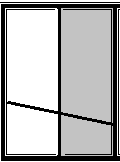
\includegraphics[scale=0.7]{figures/GAM-img1.png} & 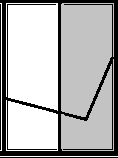
\includegraphics[scale=0.7]{figures/GAM-img2.png} & 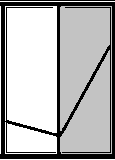
\includegraphics[scale=0.7]{figures/GAM-img3.png} & 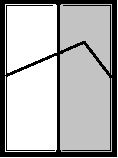
\includegraphics[scale=0.7]{figures/GAM-img4.png} \\
 \bfseries L\% & \bfseries LH\% & \bfseries H\% & \bfseries HL\%  \\
\lspbottomrule
\end{tabularx}
\caption{Schematic representation of the boundary tones.}
\label{fig:gam:1}
\end{figure}

  Another characteristic analysed was the size of the prosodic groups. Prosodic groups are those portions of texts delimited by two pauses (\citealt{Gaminde.2010,Gaminde.2012,Gaminde.2015}). One of the criteria for studying the size of these prosodic groups was the number of syllables they contained; also analysed was the total duration of the texts, the duration of the prosodic groups and the duration of the pauses.

  Finally, the speed of speech was the fourth characteristic to be taken into account. Speed was defined as the number of phonic elements, sounds and pauses that are pronounced in a specific unit of time \citep{Gil.2007}. In our case, we chose a second as a unit of time. For the number of phonic elements pronounced, although some studies use the word as a unit of measurement, we believe that the length of the word could vary significantly from one language to another, and therefore, following the criteria of previous studies  (\citealt{Gaminde.2012,Rodero.2012}), we decided that it would be more appropriate to use the syllable. It must be considered that the speed of utterance may vary even in the same reader, as it depends, among others factors, on the informative relevance of the elements that make up the speech. The speed of utterance may also reflect the speaker’s emotional state \citep{Llisterri2013}. Finally, in the studies carried out regarding speed (\citealt{Gaminde.2010,Gaminde.2012,Llisterri2013}), overall speed and speed of utterance are distinguished. Speed of utterance refers to the speed of the text taking into account the time of the pauses. In order to calculate the speed of utterance only the time of the prosodic groups is taken into account.

  Is the mother tongue a crucial feature for distinguishing some prosodic characteristics? We hypothesize that we will find evidence that there are some significant differences between the two groups of speakers, and we specifically expect there to be a difference among Spanish L1 speakers. 

  We present this work in four different sections. In the second section, following this introduction, we describe the methodology used to prepare the corpus and for the data analysis. In the third section we analyse the data based on the selected variables. Finally, in the fourth section, we summarise the main findings from the data analysis.

\section{Methodology}
\label{sec:gam:2}
  In this section we describe the methodology used to obtain the data and to process it.

  Twenty early bilingual respondents took part in the study; 10 spoke Basque as their mother tongue (Group A) while the other 10 spoke Spanish as their mother tongue (Group B). All respondents were women between the ages of 19 and 23 (\textit{m} = 20) and were educated, including at the university level, through Basque. Group A was made up of respondents from areas of the province of Biscay in which traditional varieties of Basque are spoken; they came from the following localities: Mungia, Gernika, Ibarrangelua, Markina, Ondarroa, Zamudio, Igorre, Zornotza, Durango and Berriz.\footnote{We used the official Basque names for the localities.} Group B respondents mostly come from localities outside the areas in which traditional varieties of the Basque language are spoken or from places where there has been a recent interruption in the transmission of the language. The localities selected were the following: Zalla, Santurtzi, Portugalete, Barakaldo, Bilbao (two respondents, Bilbao1 and Bilbao2), Erandio, Leioa, Sopela and Durango\footnote{Durango is the only locality where the traditional variety of Basque has a considerable presence and is transmitted normally within the family. In Bilbao, Erandio, Leioa and Sopela the transmission of the traditional variety, except in very few cases, was recently interrupted, with the majority of speakers in this town having acquired Basque within the school environment or as adults.} (see the map in \figref{fig:gam:2}). 
  
 \begin{figure}
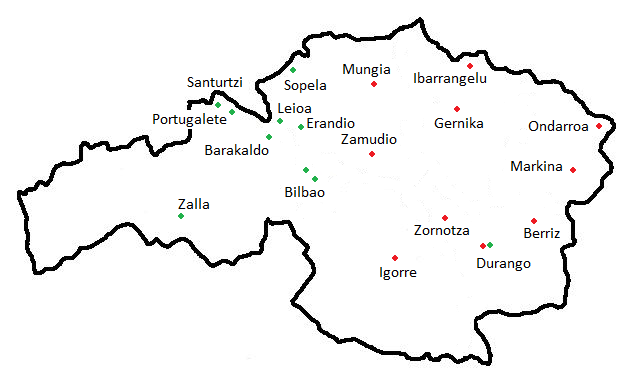
\includegraphics[scale=0.75]{figures/GAM-img5.png}
\caption{Localities of the speakers.}
\label{fig:gam:2}
\end{figure} 

As for the methodology used to gather data, we have listed some reflections on the quality of the data used when undertaking the research, especially in linguistics and more specifically in prosody. Throughout the history of linguistics, different methods have been used to obtain data on prosody: isolated words, words in context, words in phrases, words in sentences, etc. (\citealt{Gaminde.2015,Gaminde.2016}). While we find all of these ways to be acceptable, depending on the aims of the research, our view is that the language gathered using these methods is laboratory language, not real language in itself. Experienced researchers have followed this sequence of collecting data. All the ways included in this sequence however are part of the laboratory prosody. Although it is true that the majority of the words and sentences used in previous studies can be pronounced in real life, everybody is aware of some sentences that will never be used. Instead of these, we propose the use of real life sentences, or more specifically, real life texts.

Two observations should be made, one about the concept of a ``real life sentence” and the second about the ``text” concept. When we suggest the use of ``real life sentences” we are talking about sentences which can be, and are, used routinely in everyday life. In other words, we will not include an option to ask respondents to use words or sentences that they have never before used; there should be guidelines in place that require people to be asked only words and sentences that they are familiar with and would use routinely. But, as others have also done, we have also used the following types of sentences:

\protectedex{
\ea
    \label{ex:gam:1}
  \ea
  \gll Han~vendido las~ovejas de~los~hijos de~la~viuda  \\
        sold-THEY-HAVE sheep-NOM-PL sons-GEN-PL widow-GEN-SG \\
  \glt      `They have sold the sheep to the widow's sons' \\
  
   \ex 
   \gll El~amigo del~chico ha~vendido las~vacas de~la~viuda\\
        friend-NOM-SG guy-GEN-SG sold-HAS cow-NOM-PL widow-GEN-SG \\
  \glt   `The guy's friend has sold the widow's cow' \\
  \z
\z
}

In (\ref{ex:gam:1}a) there are three phrases \textit{las ovejas} `the sheepʼ, \textit{los hijos} `sonsʼ and \textit{la viuda} `widowʼ in the same sentence; the latter, \textit{viuda} `widowʼ, is dependent on the previous word, \textit{hijos} `sonsʼ, and this on the one before it, \textit{ovejas} `sheep´. In (\ref{ex:gam:1}b) there are two phrases at the beginning, \textit{amigo/chico} `guyʼ/`friendʼ, and another two at the end, \textit{viuda/vacas} `widowʼ/`cowʼ. These are not common sentences in any language, although they could be spoken in a particular situation. The fact that the researchers need to collect a concatenation of three connected phrases in (\ref{ex:gam:1}a) and two connected phrases in (\ref{ex:gam:1}b) has produced these types of sentences, which are very difficult and unusual in day-to-day language.

Even if the linguistic objectives of the research require information placed in a specific structure, we wonder about the quality of the information gathered by using these sentences and whether this kind of information can be used in a project that aspires to excellence. At the very least it could risk compromising the quality of the study. In addition, it is also known the ``methodology of observation”, without previously designed questions and following the speech of selected people. However, this kind of methodology requires much more time than asking participants interview questions. In linguistic surveys, in the majority of cases, the interest of saving time is often valued over the interest of gathering quality data. Nevertheless, even if the duration of many research projects is usually quite short, our aim is to collect data that puts respondents in their usual life contexts.

On the other hand, this contribution uses real life “texts”. Not texts created by the research team, but by an external source. In this research, a text from a journal has been selected and has been used by asking respondents to read the text aloud. Only in this way have we been able to gather the “real prosody” of the languages. Researchers making use of laboratory methodology are unable to collect data that reflects linguistic features likely to be made in authentic contexts. Using laboratory methods is an appropriate first stage for approaching an analysis of the prosody, but we believe that they should not be the only methods used, nor should they be used in the final stages of research. Laboratory methods simply do not provide glimpses of authentic everyday behaviour. 

The quality of the data our methodology allows us to collect justifies the lengthy time frame required for carrying it out. We believe that this methodology has never been used before within the context used for our study. The text given to participants to read (\ref{ex:gam:2}) was a piece of news written in Spanish that had appeared in a periodical:\footnote{\url{http://www.naiz.eus/es/actualidad/noticia/20140926/murieron-por-encima-de-sus-posibilidades-revolucion-panda-contra-la-crisis}}

\ea
  \label{ex:gam:2}
\justify \textit{La idea surge en un siquiátrico. Un grupo de personas ingresadas en un centro, afectados por una grave situación económica, deciden dar un golpe de efecto y secuestrar al presidente del Banco Central; su objetivo será cambiar el actual sistema capitalista, para que podamos volver a estar como antes. Según el director, se trata de una película hecha de modo cooperativo, financiada por muchas personas.} \\
\justify `The idea is hatched in a psychiatric hospital. A group of patients affected by a serious economic crisis decide to take a drastic measure; kidnap the president of their country's central bank. Their goal is to change the current capitalist system and return the world back to the way it was before. According to the director, the film is a cooperative project, financed by many people.ʼ \\

\z

  All the productions were recorded using a laptop with a USB microphone (Logitech PC Headset 960 USB) and the Audacity software programme \citep{AudacityTeam}.

  The Praat programme \citep{Boersma.praat} was used for the transcription, annotation and labelling of the signs (all transcriptions were made by the same researcher). On the first tier, the prosodic groups were defined and an orthographic transcription made of them. On the second tier, an open phonetic transcription was made to account for any vowel reductions found; on the same tier, label (v) was inserted, which refers to a lengthening or vowel insertion within the boundary of the prosodic group. Similarly, “H”, “L”, “LH” and “HL” are the labels that account for each type of boundary tone described in the previous section. Lastly, the “\%” label denotes the presence of a silence that delimits the prosodic group, and “\$” denotes the presence of a non-silent pause. On the third tier, all the syllables in the prosodic group were noted (\figref{fig:gam:3}).

\begin{figure}  
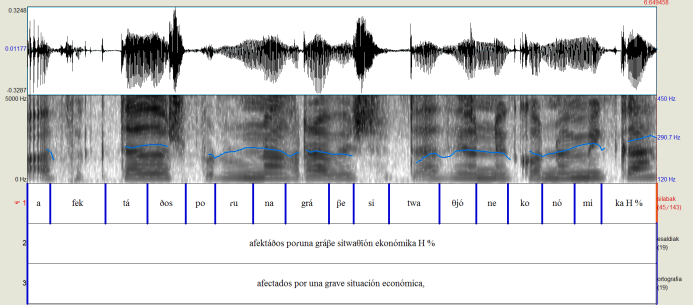
\includegraphics[width=\textwidth]{figures/GAM-img6.png}
 \caption{Example of the transcription, annotation and labelling of a sign using the Praat programme.\label{fig:gam:3}}
 \end{figure}

  Once the transcriptions were made and the corresponding labels inserted, the information was extracted by means of a script, allowing the creation of a database containing all the information recorded using the Praat programme and the information related to the respondents’ mother tongue and their localities of origin. An analysis of all these data was then carried out, which we will present in the following section. 

\section{Data analysis}
\label{sec:gam:3}

  In this section we present the analysis of the data described in the previous section. For greater expository clarity we have divided this section into four parts. In the first section we will deal with the analysis of the pauses, in the second section the boundary tones, in the third the number and length of the prosodic groups and in the fourth the production speed of the texts.

\subsection{Pauses}
\label{sec:gam:3.1}

  A total of 228 pauses were found in the analysed texts. Of these, 127 (55.7\%) were used by the respondents in Group A and 101 (44.3\%) by those in Group B. This difference was analysed using the non-parametric Mann-Whitney U test and was shown to be statistically significant (Z = -2.574; \textit{p} = 0.001), with the average range of Group A being 13.8 and Group B 7.2. 

  As we mentioned in the introduction, there are two main criteria for classifying pauses; silence or the absence thereof (±s), and the lengthening or vowel insertion at the end of the prosodic group (±v).

  The majority of the pauses analysed followed a silence (+s), 217 (95.18\%), and although we found some cases of non-silent pauses (-s), 11 (4.82\%), the percentage is very small. The differences depending on the respondents’ mother tongue are shown in \tabref{tab:gam:1}; the $\chi $\textsuperscript{2} test shows that these differences are not statistically significant ($\chi $\textsuperscript{2} = 0.295 (df = 1) \textit{p} = \textit{n.s.}).

\begin{table}
\begin{tabular}{lrd{2}rd{2}rd{2}}
\lsptoprule
& \multicolumn{2}{c}{+s} & \multicolumn{2}{c}{-s} & \multicolumn{2}{c}{Total}\\

\cmidrule(lr){2-3}\cmidrule(lr){4-5}\cmidrule(lr){6-7} & \multicolumn{1}{c}{N} & \multicolumn{1}{c}{\%} & \multicolumn{1}{c}{N} & \multicolumn{1}{c}{\%} & \multicolumn{1}{c}{N} & \multicolumn{1}{c}{\%}\\
\midrule
A &  120 &  94.49 &  7 &  5.51 &  127  & 55.7 \\
B &  97 &  96.04 &  4 &  3.96 &  101 & 44.3 \\
\lspbottomrule
\end{tabular}
\caption{Number and percentage of pauses with the presence of silence (+s) or absence of silence (-s), depending on the respondents’ mother tongue.\label{tab:gam:1}}
\end{table}

Similarly, pauses without lengthening or vowel insertion (-v) account for most of the cases studied, 196 (85.96\%), while there were 32 (14.04\%) pauses with lengthening or vowel insertion. The differences found depending on the respondents’ mother tongue are shown in \tabref{tab:gam:2}; the $\chi $\textsuperscript{2} test shows that these differences are not statistically significant ($\chi $\textsuperscript{2} = 1.175 (df = 1) \textit{p} = \textit{n.s.}).

\begin{table}

\begin{tabular}{lrd{2}rd{2}rd{2}}
\lsptoprule
& \multicolumn{2}{c}{+v} & \multicolumn{2}{c}{-v} & \multicolumn{2}{c}{Total}\\

\cmidrule(lr){2-3}\cmidrule(lr){4-5}\cmidrule(lr){6-7} & \multicolumn{1}{c}{N} & \multicolumn{1}{c}{\%} & \multicolumn{1}{c}{N} & \multicolumn{1}{c}{\%} & \multicolumn{1}{c}{N} & \multicolumn{1}{c}{\%}\\
\midrule
A &  15 &  11.81 &  112 &  88.19 &  127 & 55.7\\
B &  17 &  16.83 &  84 &  83.17 &  101 & 44.3\\
\lspbottomrule
\end{tabular}
\caption{Number and percentage of pauses with lengthening or vowel insertion (+v) or absence thereof (-v), depending on the respondents’ mother tongue. \label{tab:gam:2}}
\end{table}

\subsection{Boundary tones}

  In this section we analyse the respondents’ use of the boundary tones described in the introduction. 

  Tone L is repeated the most in all the cases, 130 (57.02\%). Tone H also had a notable frequency of appearance, 66 (28.95\%), although it is almost half that of tone L. Boundary tones LH and HL presented the lowest frequency of appearance, being 14 (6.14\%) in the case of boundary tone LH and 18 (7.89\%) in the case of HL. We can see these differences more clearly in \figref{fig:gam:4}.

\begin{figure}

\barplot{Boundary tone}{\%}{L,H,HL,LH}{
(L,57.02)
(H,28.95)
(HL,7.89)
(LH,6.14)
}
\caption{Percentage of use of each boundary tone \label{fig:gam:4}}
\end{figure}
  
  \tabref{tab:gam:3} shows the number and percentage of each boundary tone according to respondents’ mother tongue. As we can see in the table data, the speakers of both groups present a similar frequency of use, with the predominant boundary tones being L and H. The differences shown in \tabref{tab:gam:3} are not statistically significant ($\chi $\textsuperscript{2} = 1.074 (df = 3) \textit{p} = \textit{n.s.}).

\begin{table}

\begin{tabular}{lrd{2}rd{2}rd{2}}
\lsptoprule
& \multicolumn{2}{c}{A} & \multicolumn{2}{c}{B} & \multicolumn{2}{c}{Total}\\
\cmidrule(lr){2-3}\cmidrule(lr){4-5}\cmidrule(lr){6-7}
& \multicolumn{1}{c}{N} & \multicolumn{1}{c}{\%} & \multicolumn{1}{c}{N} & \multicolumn{1}{c}{\%} & \multicolumn{1}{c}{N} & \multicolumn{1}{c}{\%}\\
\midrule
L &  70 &  55.12 &  60 &  59.41 &  130 & 57.02 \\
H &  40 &  31.50 &  26 &  25.74 &  66 & 28.95 \\
HL &  9 &  7.09 &  9 &  8.91 &  18 & 7.89 \\
LH &  8 &  6.30 &  6 &  5.94 &  14 & 6.14 \\
\lspbottomrule
\end{tabular}
\caption{Number and percentage of each boundary tone depending on the respondents’ mother tongue.\label{tab:gam:3}}
\end{table}

  The greatest percentage difference depending on the respondents’ mother tongue occurs with boundary tone H. Analysing this difference using the Mann-Whitney statistical U test for two independent samples, we see that the difference is not statistically significant either (Z = -1.443; \textit{p} = \textit{n.s.}).

  Below we analyse combinations of boundary tones with different types of pauses. To do this, we used the analysis of the combinations in general to see then whether there were differences depending on the respondents’ mother tongue. In the previous section we used two parameters to characterise the four types of pauses studied; the first parameter refers to the presence or absence of silence following the prosodic group (±s), the second refers to the presence or absence of lengthening or vowel insertion (±v). From the combination of these two parameters, we can characterise the pauses as follows:

\begin{enumerate}
\item +s,+v:  Silent pause and vowel lengthening
\item -s, +v:  Non-silent pause and vowel lengthening
\item +s, -v:  Silent pause and without vowel lengthening
\item -s, -v:  Non-silent pause and without vowel lengthening
\end{enumerate}

\tabref{tab:gam:4} shows the means and standard deviations of the percentages of each combination of boundary tones associated with the different types of pauses. As shown in \tabref{tab:gam:4}, of the 16 different combinations, 4 were not recorded in any case. The combination with the highest average is that formed by boundary tone L and a silent pause and without lengthening or vowel insertion. This combination occurred in more than half the possible cases (56.04\%).

\begin{table}

 \begin{tabular}{ld{2}d{2}d{2}d{2}d{2}d{2}d{2}d{2}}
\lsptoprule
& \multicolumn{2}{c}{L} & \multicolumn{2}{c}{H} & \multicolumn{2}{c}{HL} &  \multicolumn{2}{c}{LH}\\
\cmidrule(lr){2-3}\cmidrule(lr){4-5}\cmidrule(lr){6-7}\cmidrule(lr){8-9}
&  \multicolumn{1}{c}{\={x}} &  \multicolumn{1}{c}{sd} &  \multicolumn{1}{c}{\={x}} &  \multicolumn{1}{c}{sd} &  \multicolumn{1}{c}{\={x}} &  \multicolumn{1}{c}{sd} &  \multicolumn{1}{c}{\={x}} & \multicolumn{1}{c}{sd}\\\midrule
 +s,+v &  1.08 &  3.64 &  7.72 &  8.64 &  2.80 &  5.18 &  0.25 & 1.12 \\
 -s, +v &  0.00 &  0.00 &  2.29 &  4.10 &  0.00 &  0.00 &  0.00 &  0.00\\
 +s, -v &  56.04 &  12.80 &  16.94 &  9.99 &  4.63 &  6.35 &  5.34 & 8.11\\
 -s, -v &  0.56 &  2.48 &  1.45 &  3.56 &  0.91 &  2.80 &  0.00 &  0.00\\
\lspbottomrule
\end{tabular}
\caption{Means and deviations of the percentages of each boundary tone with respect to the different types of pauses.\label{tab:gam:4}}
\end{table}

  By using as a base the frequency of each factor that influences the types of pauses and the boundary tones associated with each one, we can calculate the entire sample space as shown in \figref{fig:gam:5}.

\begin{figure}

\begin{forest}
 for tree={draw,grow=east},
 for descendants={anchor=west,child anchor=west}
 [,draw=none
 [{+}s {(}0.95{)}, no edge
  [{+}v (0.12)
    [H (0.63)]
    [L (0.11)]
    [HL (0.22)]
    [LH (0.04)]
   ]
  [{-}v (0.88)
    [H (0.22)]
    [L (0.66)]
    [HL (0.05)]
    [LH (0.07)]
  ]
 ]
  [{-}s (0.05), no edge
    [{+}v (0.45)
      [H (1)]
    ]
    [{-}v (0.55)
      [H (0.5)]
      [L (0.17)]
      [HL (0.33)]
    ]
 ]
]
\end{forest}
 
\caption{Sample space showing the different combinations of types of pauses and boundary tones.\label{fig:gam:5}}
\end{figure}

Once we have calculated the sample space, we can calculate the probability of each combination, P (C), using the following formula:

  \ea P (C) = P (±s ${\cap}$ ±v ${\cap}$ Tf)\footnote{This formula is an adaptation of the P (A ${\cap}$ B) = P(A)*P(B), known as the general formula of the probability.} \z

  Where ±s is the type of silent pause or non-silent pause, ±v is the lengthening or vowel insertion or the absence thereof and Tf is the type of boundary tone. This will give us the following expression:

  \ea P (C) = P (±s) * P (±v) * P (Tf)\z

  For example, in the case of a combination of a silent pause without vowel lengthening and a high boundary tone, we have:

 \ea P(C) = P (+s) * P (-v) * P (H)\z

  By substituting these with corresponding numerical values we obtain:

 \ea  P (C) = 0.95 * 0.88 * 0.22 = 0.184 \z

  \tabref{tab:gam:5} shows the probabilities of all the possible combinations (16) and that of all the combinations that appeared in the analysis of the texts.

\begin{table}

\begin{tabular}{ld{3}d{3}d{3}d{3}}\lsptoprule
& \multicolumn{1}{c}{L}& \multicolumn{1}{c}{H} & \multicolumn{1}{c}{HL} & \multicolumn{1}{c}{LH}\\\midrule
+s, +v &  0.013 &  0.072 &  0.025 &  0.005\\
-s, +v &  0.000 &  0.023 &  0.000 &  0.000\\
+s, -v &  0.552 &  0.184 &  0.042 &  0.059\\
-s, -v &  0.004 &  0.011 &  0.007 &  0.000\\

\lspbottomrule
\end{tabular}
\caption{Probabilities of each combination of boundary tone with the different types of pauses.\label{tab:gam:5}}
\end{table}

  To present the results based on the respondents’ mother tongue the information will be broken down by each type of boundary tone. In this way, \tabref{tab:gam:6} shows the results corresponding to the combinations of boundary tone L. The differences that appear in the table are not statistically significant according to the Mann-Whitney statistical U test. Furthermore, although the respondents of both groups used the same number of combinations these were not the same.

\begin{table}

\begin{tabular}{ld{2}d{2}d{2}d{2}}
\lsptoprule
& \multicolumn{2}{c}{A} &  \multicolumn{2}{c}{B}\\
\cmidrule(lr){2-3}\cmidrule(lr){4-5}
&  \multicolumn{1}{c}{\={x}} &  \multicolumn{1}{c}{sd} &  \multicolumn{1}{c}{\={x}} &  \multicolumn{1}{c}{sd}\\
\midrule
 +s,+v  &  2.16   &  5.04 &  0.00 &  0.00\\
 -s, +v &  0.00      &  0.00    &  0.00 &  0.00\\
 +s, -v &  53.36  &  9.39 &  58.71 &  15.50\\
 -s, -v &  0.00      &  0.00    &  1.11 &  3.51\\
\lspbottomrule
\end{tabular}
\caption{Means and deviations of the percentages of boundary tone L with respect to the different types of pauses depending on the respondents’ mother tongue.\label{tab:gam:6}}
\end{table}

  The data on the combinations of boundary tone H is shown in \tabref{tab:gam:7}. The differences shown in the table are not statistically significant according to the Mann-Whitney statistical U test. It was observed that one combination less was used among the respondents in Group B.

\begin{table}

\begin{tabular}{ld{2}d{2}d{2}d{2}}
\lsptoprule
& \multicolumn{2}{c}{A} &  \multicolumn{2}{c}{B}\\\cmidrule(lr){2-3}\cmidrule(lr){4-5}
&  \multicolumn{1}{c}{\={x}} &  \multicolumn{1}{c}{sd} &  \multicolumn{1}{c}{\={x}} &  \multicolumn{1}{c}{sd}\\\midrule
 +s,+v &  4.46 &  6.47 &  10.97 & 9.59 \\
 -s, +v &  2.68 &  4.35 &  1.91 & 4.03\\
 +s, -v &  21.08 &  10.40 &  12.79 & 7.98\\
 -s, -v &  2.91 &  4.69 &  0.00 & 0.00\\
\lspbottomrule
\end{tabular}
\caption{Means and deviations of the percentages of boundary tone H with respect to the different types of pauses depending on the respondents’ mother tongue.\label{tab:gam:7}}
\end{table}

  The results from the combinations of boundary tone HL are shown in \tabref{tab:gam:8}. The differences that appear in the table according to the Mann-Whitney U test are not statistically significant in any case. Here the respondents of both groups use the same combinations. 

\begin{table}

\begin{tabular}{ld{2}d{2}d{2}d{2}}
\lsptoprule
& \multicolumn{2}{c}{A} &  \multicolumn{2}{c}{B}\\\cmidrule(lr){2-3}\cmidrule(lr){4-5}
&  \multicolumn{1}{c}{\={x}} &  \multicolumn{1}{c}{sd} &  \multicolumn{1}{c}{\={x}} &  \multicolumn{1}{c}{sd}\\\midrule
 +s,+v &  1.67 &  5.27 &  3.93 & 5.10\\
 -s, +v &  0.00 &  0.00 &  0.00 & 0.00\\
 +s, -v &  5.33 &  6.30 &  3.93 & 6.66\\
 -s, -v &  0.91 &  2.90 &  0.91 & 2.90\\
\lspbottomrule
\end{tabular}
\caption{Means and deviations of the percentages of boundary tone HL with respect to the different types of pauses depending on the respondents’ mother tongue.\label{tab:gam:8}}
\end{table}

  Finally, the results from the combinations of boundary tone LH are shown in \tabref{tab:gam:9}. The differences that appear in the table according to the Mann-Whitney U test are not statistically significant in any case. In this case, the respondents in Group B used just one combination from all the possible combinations.

\begin{table}

\begin{tabular}{ld{2}d{2}d{2}d{2}}
\lsptoprule
& \multicolumn{2}{c}{A} &  \multicolumn{2}{c}{B}\\\cmidrule(lr){2-3}\cmidrule(lr){4-5}
&  \multicolumn{1}{c}{\={x}} &  \multicolumn{1}{c}{sd} &  \multicolumn{1}{c}{\={x}}  &  \multicolumn{1}{c}{sd}\\\midrule
 +s,+v &  0.5 &  1.58 &  0.00 & 0.00\\
 -s, +v &  0.00 &  0.00 &  0.00 & 0.00\\
 +s, -v &  4.93 &  7.66 &  5.75 & 8.94\\
 -s, -v &  0.00 &  0.00 &  0.00 & 0.00\\
\lspbottomrule
\end{tabular}
\caption{Means and deviations of the percentages of boundary tone LH with respect to the different types of pauses depending on the respondents’ mother tongue.\label{tab:gam:9}}
\end{table}

  As shown in the previous analyses, there are no statistically significant differences depending on the respondents’ mother tongue in terms of the percentages of each combination of the boundary tones with the different types of pauses. The only notable difference is that, of the 16 possible combinations, the respondents in Group A used 11 while the respondents in Group B used only 9.

\subsection{Prosodic groups} 

  In this section we analyse the number of prosodic groups the respondents form in the texts and the length of these groups. As already indicated in the introduction, a prosodic group is defined as the segment of speech between two pauses. To study the length of the texts, we took into account the number of syllables contained in each group, the total duration of the groups, the duration of the prosodic groups in each text, without taking into account the duration of the pauses, and finally, the duration of all the pauses in each text.

  In the 20 texts analysed, a total of 228 prosodic groups were accounted for. This equates to an average of 11.4 prosodic groups per text (sd = 2.6). If we look at the minimum and maximum number of groups formed by the respondents we see that the respondent who formed the least number of prosodic groups and who, therefore, used the fewest pauses and presumably read the text faster and more fluidly that the others, formed 9 prosodic groups. In contrast, the respondent who divided the text into the highest number of prosodic groups formed 20 in reading the text.

  On average, the respondents in Group A, those with Basque as their mother tongue, formed the most prosodic groups for each text, 12.7 (sd = 3.13); those in Group B, i.e. those with Spanish as their mother tongue, had an average of 10.1 (sd = 0.88). According to the Mann-Whitney U test this difference is statistically significant (Z = -2.574, \textit{p} = 0.010), with the respondents in Group A having an average of 13.8 and the respondents in Group B an average of 7.2.

  If we analyse the number of syllables in each prosodic group we see that this ranges from 2 syllables in the shortest prosodic groups to 23 in the longest. The average number of syllables per group is 11.85 (sd = 5.01). Analysing this data based on the respondents’ mother tongue we see that those in Group A have an average of 10.66 (sd = 4.83) for each prosodic group (ranging between 2 and 23). The respondents in Group B have an average of 13.35 (sd = 4.88, ranging between 3 and 23). We can conclude that the respondents in Group B use a greater number of syllables for each prosodic group than the respondents in Group A. As the data gathered for this analysis correspond with the assumptions of the T test, we applied this treatment to see whether the differences were statistically significant. Therefore, assuming equal variances extracted from the application of the Levene test, the difference in the length of the prosodic groups based on the respondents’ mother tongue is statistically significant (T= 4.158 (df = 1.226) p < 0.001).

  The average total duration of the texts, including both the duration of the prosodic groups and the duration of the pauses, is 21.765 ms (sd = 2497.95). The respondents in Group A present an average of 22.422 ms (sd = 2864.34), the average of the respondents in Group B is 21.108 ms (sd = 1975.83). Although the average of the respondents of Group A is higher than that of Group B, the difference is not statistically significant according to the Mann-Whitney U test (Z = -1.098, \textit{p} = \textit{n.s.}).

  If we only analyse the duration of the prosodic groups, that is, discounting the time of the pauses, we obtain an overall average of 18,811 ms for each text (sd = 1891.81). The average of the respondents in Group A is 19.498 ms (sd = 2180.81) and that of the respondents in Group B is 18.123 ms (sd = 1322.58). The differences are not statistically significant according to the Mann-Whitney U test (Z = -1.209, \textit{p} = \textit{n.s.}), the average range being 12.10 for the respondents in Group A and 8.90 for those in Group B.

  With respect to the duration of the pauses, the overall average of these for each text is 2936 ms (sd = 931.01). The average of the respondents in A is 2924 ms (sd = 1102.93) and that of the respondents in Group B is 2947 ms (sd = 783.01). The differences are not statistically significant according to the Mann-Whitney U test (Z = -0,227, \textit{p} = \textit{n.s.}), the average range being 10.20 for the respondents in Group A and 10.80 for those in Group B.

\subsection{Speed of text production}

  As already indicated in the introduction, by performing an analysis of the speed we can calculate the overall speed, taking into account the complete time of the text; that is, the time of the prosodic groups and that of the pauses and speed of utterance, discounting the time of the pauses.

  The average overall speed, expressed in syllables per second, is 7.25 (sd = 0.66). When we analyse the data based on the respondents’ mother tongue, we can see that the respondents in Group B read faster, 7.47 (sd = 0.53), than the respondents in Group A, 7.02 (sd = 0.73). The differences are not statistically significant according to the Mann-Whitney U test (Z = -1.324, \textit{p} = \textit{n.s.}); the average range being 8.75 for the respondents in Group A and 12.25 for those in Group B.

  The data obtained for speed of utterance show an overall average of 6.28 syllables per second (sd = 0.648). When we analyse the data based on the respondents’ mother tongue we again find a higher average among the respondents in Group B, 6.44 (sd = 0.581), while the average of the respondents in Group A is 6.12 (sd = 0.702) syllables per second. The differences are not statistically significant according to the Mann-Whitney U test (Z = -0,945, \textit{p} = \textit{n.s.}); with the average range being 9.25 for the respondents in Group A and 11.75 for those in Group B.

  It would be interesting to observe whether the speed and the number of pauses are correlated in some way. In general, according to the Pearson correlation, there is a negative correlation of -0.625 (\textit{p} = 0.003) between the overall speed and the number of pauses, and -0.658 (\textit{p} = 0.002) when we analyse the correlation between the speed of utterance and the number of pauses. This correlation can be described as reasonable, because it is between 0,5 and 0,7 \citep{HerreraSoler.2011}.

  Basing the analysis on the respondents’ mother tongue we obtained the data shown in \tabref{tab:gam:10}, for the overall speed (os) and for speed of utterance (su). The correlation is very strong in the case of the respondents in Group A, especially when the number of pauses is correlated with the speed of utterance, and is somewhat less with the overall speed, and these correlations are statistically significant. In the case of the respondents in Group B there is some correlation when the number of pauses is correlated with the speed of utterance, but there is almost no correlation in the case of overall speed; in any event, these correlations are not statistically significant.  

\begin{table}

\begin{tabular}{ld{3}d{3}d{3}d{3}}
\lsptoprule
& \multicolumn{2}{c}{os} &  \multicolumn{2}{c}{su}\\\cmidrule(lr){2-3} \cmidrule(lr){4-5}
&  \multicolumn{1}{c}{r} & \multicolumn{1}{c}{p} &  \multicolumn{1}{c}{r} & \multicolumn{1}{c}{p}\\\midrule
A &  -0.699 &  0.028 &  -0.814 & 0.004\\
B &  0.095 &  \textit{n.s.} &  -0.605 & \textit{n.s.}\\
\lspbottomrule
\end{tabular}
\caption{Correlations between the overall speed (os) and the speed of utterance (su) with the number of pauses in the texts\label{tab:gam:10}}
\end{table}

\section{Discussion}
The methodology chosen for this study has yielded findings that are more reliable than those of other studies because the data and the methodology we have used are closer to the linguistic or prosodic realizations of real life. The closer studies can come to presenting authentic situations, of the type found in field studies, the more reflective the results of these are of non-observed data, and consequently the results are more reliable from a linguistic point of view. There are however occasions when working within real-life situations is not possible. At these times, work must be carried out in artificial contexts when observation of certain types of language is necessary for the aims of the study.

The use of real texts instead of unrelated sentences places the prosodic features in their context. By using texts instead of isolated words, respondents do not presuppose anything and they act in a way that comes much closer to the way they would in real life. Therefore, the linguistic features participants produce when reading come closer to those made in authentic utterances than they do when participants read language within fictitious contexts. Additionally, the use of real texts encourages participants to focus on the meaning of what they are reading and makes them less conscious of how they are going to pronounce the sentence.  

By using texts, researchers also have the opportunity to measure other acoustic features, such as pauses or the speed of text reproduction. This is important when analysing productions of people with different mother tongues.

It is still too early to understand the differences between the traditional methods used to gather prosodic data and the method we propose in this work. Comparisons between the two methods must be made however to improve the quality of the data collected and consequently, the quality of the results.

In general, and taking into account the research hypothesis, we can conclude that the mother tongue of early bilingual speakers influences certain characteristics in read texts, such as the fact that the respondents in Group B read more quickly, forming a lower number of prosodic groups for each text and a greater number of syllables for each prosodic group. In any case, in a large number of the characteristics studied we did not encounter statistically-significant differences. It is important to note that the results of the acoustic analysis of this material allow comparisons to be made between the prosodic features of Spanish L1 and Basque L1 speakers. These results, which are in line with previous findings of bilingual studies for other languages, show that speakers who have Basque as L1 tend to read at a lower rate, inserting more pauses than Spanish L1 speakers.


\section{Conclusions}

  In this final section we summarise the main findings extracted from the analyses of the data described in the previous section.

  With regard to the pauses, it was shown that in these types of texts silent pauses predominate (95.18\%) and without lengthening or vowel insertion at the end (85.96\%); it is also clear that there are no statistically significant differences as regards the type of pause selected based on the respondents’ mother tongue. On the contrary, it was shown that the respondents in Group A made a greater number of pauses than those in Group B, this difference being statistically significant. In our opinion it is because the used test is neither in their mother tongue nor in the school language.

  Regarding the boundary tones, it was evident that the most predominant were the single tones and, among these, boundary tone L had the highest frequency. Based on the respondents’ mother tongue, no statistically significant differences were detected, the percentages of use being similar in both groups of respondents. With respect to the possible combinations of the boundary tones and different types of pauses, the combination used in the majority of cases is formed by boundary tone L and a pause made with silence at the end of a prosodic group and without lengthening or vowel insertion, the probability associated with this combination being 0.552. As regards the possible differences based on the respondents’ mother tongue, we found that these were not statistically significant.

  As regards the number of prosodic groups formed per text, we found a statistically significant difference between the respondents in both groups; the number of prosodic groups per text used by the respondents in Group A was higher. This difference correlates, obviously, with the number of pauses.

  We saw that the number of syllables per prosodic group was higher among the respondents in Group B, this being a statistically significant difference. It is due to the fact that the language used for the test was the participants' mother tongue, thus they were better able to create longer prosodic groups.

  As regards the overall duration of the texts we observed that the respondents in Group A took longer to read the texts and the same occurred with the average duration of the prosodic groups and the pauses. Despite this, the differences in duration were not statistically significant in any of the three cases. It is worth noting the large standard deviation shown by the respondents in Group A with respect to the duration of the pauses, which suggests a greater dispersion of data.

 With regard to speed, we observed that, although not statistically significant, the speakers in Group A read more slowly than those in Group B, both in terms of overall speed and the speed of utterance. Moreover, we saw that there was a negative correlation between the speed and the number of pauses, stronger among the speakers in Group A; and there is also negative correlation between the speed of utterance and number of pauses.

  We are aware of the limitations of our research. Firstly, the limited number of respondents who were part of the sample group. Secondly, it would be necessary to select a text produced in Basque so that it could be read under the same conditions, followed by observations and comparisons of any implications. Thirdly, it is necessary to focus on research that deals with prosodic aspects in texts, whether these are spontaneous or read.


\printbibliography[heading=subbibliography,notkeyword=this]

\end{document}